\chapter{Concept}
\label{chap:concept}

%\todo{Malware }

\section{Introduction}

\begin{figure}[h]
    \centering
    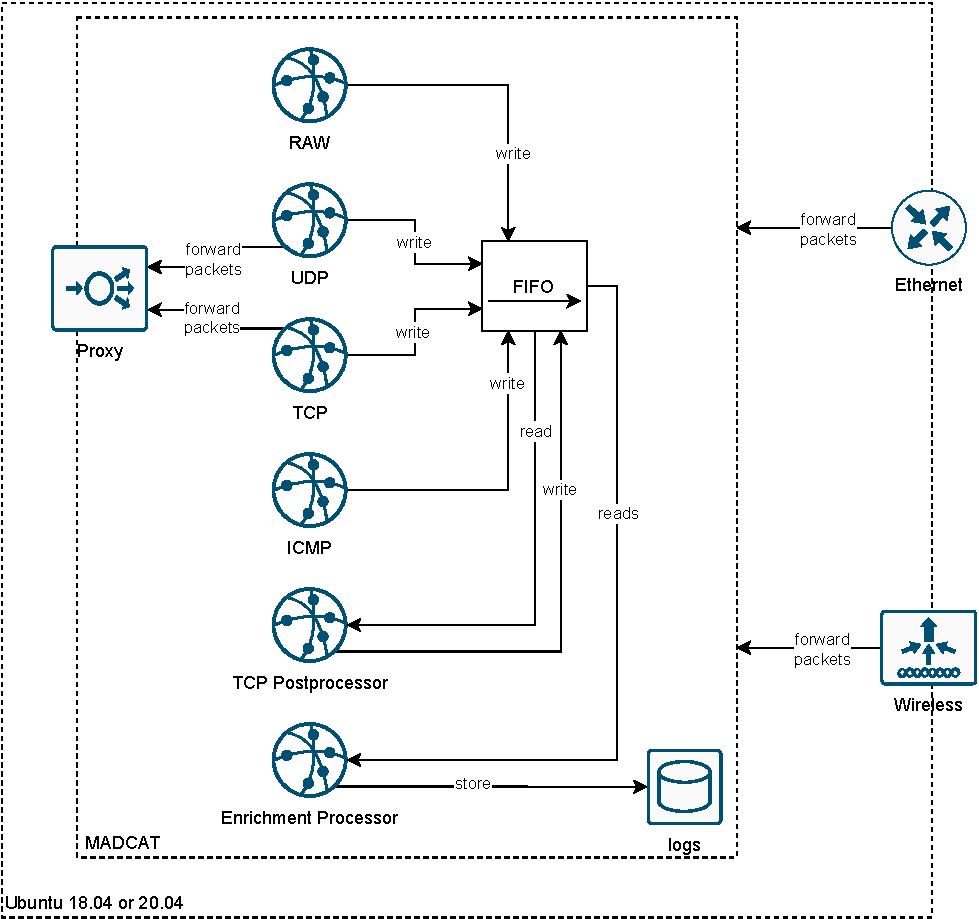
\includegraphics[width=\textwidth]{figures/heicat-architecture.pdf}
    \caption[Honeytrap results]{Honeytrap results}
    \label{fig:madcat-architecture}
\end{figure}

\begin{figure}[h]
    \centering
    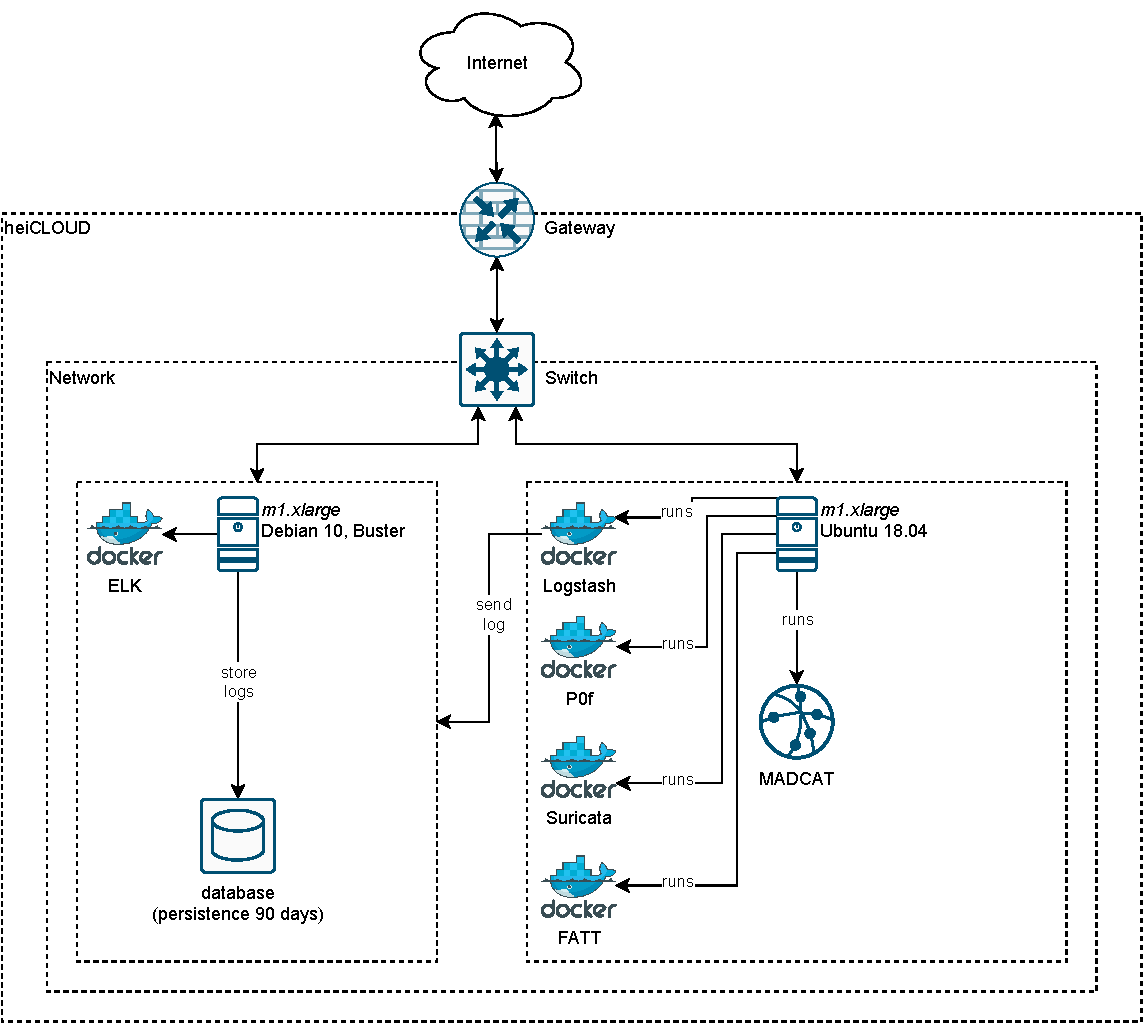
\includegraphics[width=\textwidth]{figures/heicat-conecpt.pdf}
    \caption[Honeytrap results]{Honeytrap results}
    \label{fig:madcat-architecture}
\end{figure}

%\section{Methods Used}

%\subsection{Requirements and specification}

%\subsection{Proposed Honeypots}

%\subsubsection{Cowire}

%\subsubsection{Dionaea}

%\todo{2 weitere Honeypots fuer Datenauswertung}

%\subsubsection{Honeyd}

%\subsection{Configuration Honeyd}

%\subsection{Frameworks and technologies}

%\subsubsection{HoneyTrap}

%\section{Architecture}

%\todo{Maybe rename section}

%\section{Data Management}

%\section{Data Analysis}

\section{Summary}